

\section{ELF format (64 bits)}

The {\bf Executable and Linkable Format (ELF)} is the default
binary format on Linux-based systems.  ELF is used for executable files, object
files, shared libraries, and core dumps.

The 32-bit format is similar, differing mainly in the size and order of certain
header fields and other data structures.

ELF binaries really consist of only four types of components: 
\begin{itemize}
        \item an executable header
        \item a series of (optional) program headers
        \item a number of sections
        \item and a series of (optional) section headers, one per section.
\end{itemize}

\subsection{The Executable Header}
It is just a structured series of bytes telling you that it’s an ELF file, what
kind of ELF file it is, and where in the file to find all the other contents.

To find out what the format of the executable header is, you can look up its
type definition (and the definitions of other ELF-related types and constants)
in \verb+/usr/include/elf.h+ or in the ELF specification.

\begin{verbatim}
readelf -e <binary>
\end{verbatim}

\subsection{Section Headers and sections}
The code and data in an ELF binary are logically divided into contiguous
nonoverlapping chunks called {\bf sections}. often a section is nothing more
than an unstructured blob of code or data. Every section is described by a {\bf
section header}, which denotes the properties of the section and allows you to
locate the bytes belonging to the section. The section headers for all sections
in the binary are contained in the i{\bf section header table}.

The division into sections is intended to provide a convenient organization for
use by the linker. Therefore the section header table is an optional part of
the ELF format.

To load and execute a binary in a process, you need a different organization
of the code and data in the binary. For this reason, ELF executables specify
another logical organization, called {\bf segments}, which are used at execution time
(as opposed to sections, which are used at link time). 


Typical ELF files that you’ll find on a GNU/Linux system are organized into a series of standard (or de facto standard) sections


\begin{verbatim}
readelf --sections --wide <binary>
\end{verbatim}

\begin{itemize}
    \item \verb+.init+: executable code that performs initialization tasks and needs to run before any other code in the binary is executed.
    \item \verb+.fini+: it runs after the main program completes, essentially functioning as a kind of destructor.

    \item \verb+.text+: is where the main code of the program resides
    \item \verb+.bss+, \verb+.data+, and \verb+.rodata+i (read-only-data): 
    \item \verb+plt+, \verb+.got+ and \verb+.got.plt+: are related to lazy
        binding.
    \item \verb+.rel.*+ and \verb+.rela.*+ (\verb+readelf --relocs+): contain
        information used by the linker for performing relocations.
    \item \verb+.dynamic+: unctions as a “road map” for the operating system
        and dynamic linker when loading and setting up an ELF binary for
        execution.

    \item \verb+.init_array and .fini_array+: ontains an array of pointers to
        functions to use as constructors (destructor). Each of these functions
        is called in turn when the binary is initialized, before main is
        called.
    \item \verb+.shstrtab, .symtab, .strtab, .dynsym, and .dynstr+: 
\end{itemize}

\subsection{Program Headers}
The program header table provides a segment view of the binary, as opposed to
the section view provided by the section header table,  is used by the
operating system and dynamic linker when loading an ELF into a process for
execution to locate the relevant code and data and decide what to load into
virtual memory.

An ELF segment encompasses zero or more sections, essentially bundling these
into a single chunk. Since segments provide an execution view, they are needed
only for executable ELF files and not for nonexecutable files such as
relocatable objects.
\begin{verbatim}
readelf --wide --segments <binary>
\end{verbatim}

\subsection{Lazy Binding, PLT and GOT}
Lazy binding ensures that the dynamic linker never needlessly wastes time on
relocations; it only performs those relocations that are truly needed at
runtime. On Linux, lazy binding is the default behavior of the dynamic linker.


Lazy binding in Linux ELF binaries is implemented with the help of two special
sections, called the {\bf Procedure Linkage Table} (\verb+.plt+) and the {\bf
Global Offset Table} (\verb+.got+).  ELF binaries often contain a separate GOT
section called \verb+.got.plt+ for use in conjunction with \verb+.plt+ in the
lazy binding process. The \verb+.got.plt+ section is analogous to the regular
\verb+.got+, and for your purposes here, we can consider them to be the same
(in fact, historically, they were).

the following figure illustrates the lazy binding process and the role of the
PLT and GOT.


 \begin{figure}
  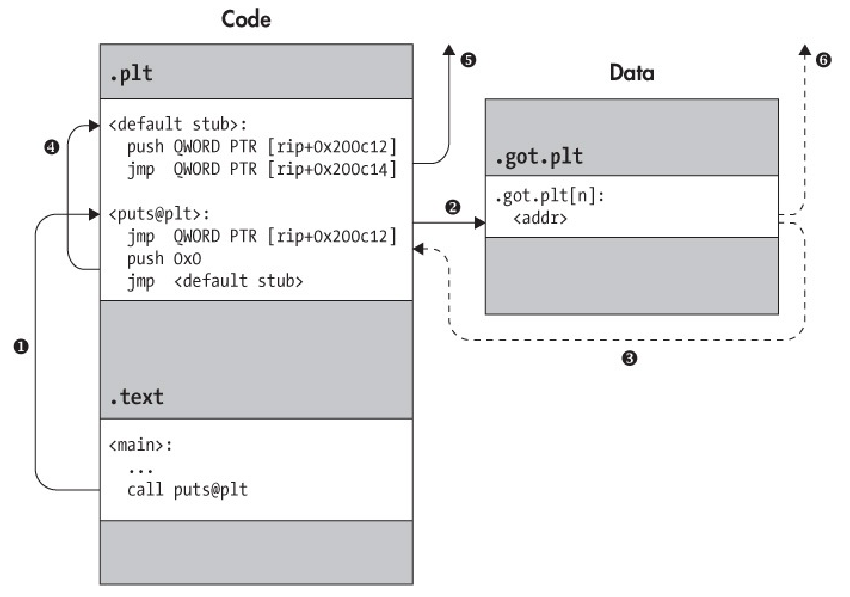
\includegraphics[width=\linewidth]{binary/anatomy/images/lazy_binding.png}
  \caption{Calling a shared library function via PLT}
  \label{fig:lazy_binding}
\end{figure}

As the figure (and a \verb+readelf --sections --wide+ output) show, \verb+.plt+
is a code section that contains executable code while \verb+.got.plt+ is a data
section.

The PLT consists entirely of stubs of a well-defined format, dedicated to
directing calls from the \verb+.text+ section to the appropriate library
location. To explore the format of the PLT, let’s look at a disassembly of the
\verb+.plt+ section from the example binary, as shown in Listing 2-7. (The instruction opcodes have been omitted for brevity.) Listing 2-7: Disassembly of a .plt section


\begin{verbatim}
$ objdump -M intel --section .plt -d a.out
a.out: file format elf64-x86-64

Disassembly of section .plt:

00000000004003f0 <puts@plt-0x10>:
4003f0: push QWORD PTR [rip+0x200c12] # 601008 <_GLOBAL_OFFSET_TABLE_+0x8>
4003f6: jmp QWORD PTR [rip+0x200c14] # 601010 <_GLOBAL_OFFSET_TABLE_+0x10>
4003fc: nop DWORD PTR [rax+0x0]

0000000000400400 <puts@plt>:
400400: jmp QWORD PTR [rip+0x200c12] # 601018 <_GLOBAL_OFFSET_TABLE_+0x18>
400406: push 0x0
40040b: jmp 4003f0 <_init+0x28>

0000000000400410 <__libc_start_main@plt>:
400410: jmp QWORD PTR [rip+0x200c0a] # 601020 <_GLOBAL_OFFSET_TABLE_+0x20>
400416: push 0x1
40041b: jmp 4003f0 <_init+0x28>
\end{verbatim}

the first stub is a default stub. After comes a stub for each library function
following the same pattern. Note that for each consecutive function stub, the
value pushed onto the stack, which is incremented, is an identifier.


\subsubsection{Dynamic Resolution of a Library Function Using the PLT}

Let’s say the prgramm wants to call the \verb+puts+ function of the \verb+libc+
library. Instead of calling it directly, a call is made to to the corresponding
PLT stub, \verb+puts@plt+.


The PLT stub begins with an indirect jump instruction, which jumps to an
address stored in the \verb+.got.plt+ section (step 2 of
figure~\ref{fig:lazy_binding}). Initially, before the lazy binding has
happened, this address is simply the address of the next instruction in the
function stub, which is a push instruction. Thus, the indirect jump simply
transfers control to the instruction directly after it (step 3 of
figure~\ref{fig:lazy_binding})! That’s a rather roundabout way of getting to
the next instruction, but there’s a good reason for doing it this way.

The push instruction pushes an integer (in this case, \verb+0x0+) onto the
stack. As mentioned, this integer serves as an identifier for the PLT stub in
question.  Subsequently, the next instruction jumps to the common default stub
shared among all PLT function stubs (step 4 of figure~\ref{fig:lazy_binding}).
The default stub pushes another identifier (taken from the GOT), identifying
the executable itself, and then jumps (indirectly, again through the GOT) to
the {\bf dynamic linker} (step 5 of figure~\ref{fig:lazy_binding}).

Using the identifiers pushed by the PLT stubs, the dynamic linker figures out
that it should resolve the address of \verb+puts+ and should do so on behalf of
the main executable loaded into the process. This last bit is important because
there may be multiple libraries loaded in the same process as well, each with
their own PLT and GOT. The dynamic linker then looks up the address at which
the \verb+puts+ function is located and plugs the address of that function into
the GOT entry associated with \verb+puts@plt+. Thus, the GOT entry no longer
points back into the PLT stub, as it did initially, but now points to the
actual address of \verb+puts+. At this point, the lazy binding process is
complete.

Finally, the dynamic linker satisfies the original intention of calling
\verb+puts+ by transferring control to it. For any subsequent calls to
\verb+puts@plt+, the GOT entry already contains the appropriate (patched)
address of \verb+puts+ so that the jump at the start of the PLT stub goes
directly to \verb+puts+ without involving the dynamic linker (step 6 of
figure~\ref{fig:lazy_binding})

\subsubsection{Why Use a GOT?}
At this point, you may wonder why the GOT is needed at all. For example,
wouldn’t it be simpler to just patch the resolved library address directly into the
code of the PLT stubs? 

One of the main reasons boils down to {\bf security}. If there’s a
vulnerability in the binary somewhere, it would be easy for an attacker to
modify the code of the binary if executable sections like \verb+.text+ and
\verb+.plt+ were writable. But because the GOT is a data section and it’s okay
for it to be writable, it makes sense to have the additional layer of
indirection through the GOT.  While an attacker may still succeed in changing
the addresses in the GOT, this attack model is a lot less powerful than the
ability to inject arbitrary code.

The other reason has to do with code shareability in shared libraries. As
discussed, modern operating systems save  memory by sharing the code of
libraries among all processes using them. That way, instead of having to load a
separate copy of every library for each process using it, the operating system
has to load only a single copy of each library. However, even though there is
only a single physical copy of each library, the same library will likely be
mapped to a completely different virtual address for each process. The
implication is that you can’t patch addresses resolved on behalf of a library
directly into the code because the address would work only in the context of
one process and break the others. Patching them into the GOT instead does work
because each process has its own private copy of the GOT.

References from the code to relocatable data symbols (such as variables and
constants exported from shared libraries) also need to be redirected via the
GOT to avoid patching data addresses directly into the code. The difference is
that data references go directly through the GOT, without the intermediate step
of the PLT. This also clarifies the distinction between the \verb+.got+ and
\verb+.got.plt+ sections: \verb+.got+ is for references to data items, while
\verb+.got.plt+ is dedicated to storing resolved addresses for library
functions accessed via the PLT.






